\documentclass[tikz,border=5pt]{standalone}
\usepackage{amsmath,amssymb}
\begin{document}
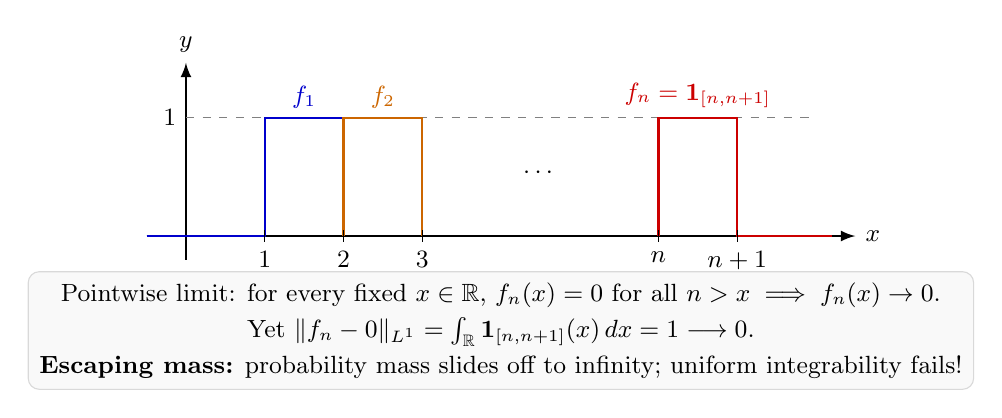
\begin{tikzpicture}[>=latex, font=\small]
  \draw[->, thick] (-0.5, 0) -- (8.5, 0) node[right] {$x$};
  \draw[->, thick] (0, -0.3) -- (0, 2.2) node[above] {$y$};

  \node[left] at (0, 1.5) {$1$};
  \draw[dashed, gray] (0, 1.5) -- (8, 1.5);

  % f_1
  \draw[thick, blue!80!black] (-0.5, 0) -- (1, 0) -- (1, 1.5) -- (2, 1.5) -- (2, 0);
  \node[blue!80!black, above] at (1.5, 1.5) {$f_1$};

  % f_2
  \draw[thick, orange!80!black] (2, 0) -- (2, 1.5) -- (3, 1.5) -- (3, 0);
  \node[orange!80!black, above] at (2.5, 1.5) {$f_2$};

  \node at (4.5, 0.8) {$\cdots$};

  % f_n
  \draw[thick, red!80!black] (6, 0) -- (6, 1.5) -- (7, 1.5) -- (7, 0) -- (8.2, 0);
  \node[red!80!black, above] at (6.5, 1.5) {$f_n = \mathbf{1}_{[n, n+1]}$};

  \foreach \x/\lbl in {1/1, 2/2, 3/3, 6/n, 7/n+1} {
    \draw (\x, 2pt) -- (\x, -2pt) node[below] {$\lbl$};
  }

  \node[align=center, fill=gray!5, draw=gray!30, rounded corners, inner sep=4pt] at (4.0, -1.2)
    {Pointwise limit: for every fixed $x \in \mathbb{R}$, $f_n(x) = 0$ for all $n > x \implies f_n(x) \to 0$.\\[2pt]
     Yet $\|f_n - 0\|_{L^1} = \int_{\mathbb{R}} \mathbf{1}_{[n, n+1]}(x)\,dx = 1 \centernot\longrightarrow 0$.\\[2pt]
     \textbf{Escaping mass:} probability mass slides off to infinity; uniform integrability fails!};
\end{tikzpicture}
\end{document}
